\documentclass{beamer} %
\usetheme{Dresden}
\usecolortheme{beaver}
\usepackage[portuguese]{babel}
\usepackage[utf8x]{inputenc}
\usefonttheme{professionalfonts}
\usepackage{times}
\usepackage{tikz}
\usepackage{amsmath}
\usepackage{tabulary}
\usepackage{pgfgantt}
\usepackage{verbatim}
\usetikzlibrary{arrows,shapes}
\usepackage{adjustbox}
\usepackage{soul}
\usepackage{listings}
\usepackage{adjustbox}
\setbeamertemplate{itemize item}{\color{red}$\blacksquare$}
\usepackage{hyperref}
\title{avance1}


\newtheorem{defi}{Definição}
\newtheorem{lema}{Lema}
\newtheorem{teo}{Teorema}
\newtheorem{prop}{Proposição}
\newtheorem{prova}{Demonstração}
\newtheorem{exemplo}{Exemplo}
\newtheorem{hipotese}{Hipótese}
\newtheorem{algo}{Algoritmo}
\newcommand{\R}{\mathbb{R}}
%\newcommand{\P}{\mathcal{P}}
\newcommand{\C}{\mathcal{C}}
\newcommand{\I}{\mathcal{I}}
\newcommand{\A}{\mathcal{A}}
\newcommand{\F}{\mathcal{F}}
\newcommand{\X}{\mathcal{X}}
\newcommand{\Y}{\mathcal{Y}}
\newcommand{\M}{\mathcal{M}}
\newcommand{\E}{\mathbb{E}}
\newcommand{\V}{\mathbb{V}}
\newcommand{\Prob}{\mathbb{P}}
\newcommand{\1}{\mathbb{I}}

\title{Computação de Efeitos Marginais em Florestas Aleatórias}
\institute[]{Universidade Federal Fluminense}
\author{Pedro Cavalcante Oliveira}

\date{\today}

\begin{document}
\tikzstyle{every picture}+=[remember picture]
\lstset{language=C++}   
\everymath{\displaystyle}

\begin{frame}

	\titlepage
\end{frame}

%------------------------------------------------------



\begin{frame}
A previsão $\hat{y}$ é a constante  $\beta_0$ e o produto interno entre o vetor com explicativas e o de parâmetros estimados.

\begin{align}
    \hat{y} = \beta_0 + \sum_{i=1}^{k} \beta_i \mathbf{x}_i 
\end{align}

Implicando que o efeito marginal de uma variável é constante na própria variável e independe do nível das outras.
\end{frame}



\begin{frame}
\begin{itemize}
    \item É possível adicionar funções não-lineares dos regressores originais para remediar esse problema
    \item Ao custo de perder precisão na estimação dos parâmetros proporcionalmente ao número de adições
    \item Algumas classes de modelos contornam esse tipo de limitação
    \item Árvores de Decisão, por exemplo
\end{itemize}
\end{frame}





\begin{frame}
Pode-se elaborar uma série de perguntas sobre a observações em questão e designar à cada possível combinação de respostas uma regra de previsão ou classificação. 

\BlankLine
\BlankLine
\BlankLine

Isso pode ser representado por uma série de bifurcações conectadas, um \textbf{grafo árvore.}
\end{frame}


\begin{frame}

\begin{figure}[H]
    \centering
    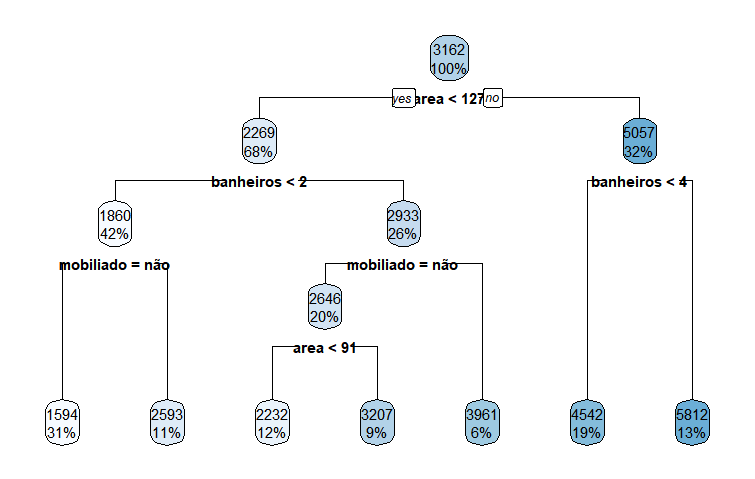
\includegraphics[scale = .55]{imagens/arvore_decisao_houses.png}
    \caption{Um exemplo de árvore de regressão. Elaboração própria.}
    \label{fig:arvore_reg}
\end{figure}
\end{frame}




\begin{frame}
Surge uma questao: como escolher testes, em qual ordem e com quais parametros? Escolha a pergunta cuja resposta maximiza alguma métrica de qualidade.

\begin{itemize}
    \item \textbf{Classificação:} Impureza de Gini entre classes, Ganho de Informação 
    \item \textbf{Regressão:} Diferença de média entre grupos, soma ponderada das variâncias da variável resposta em cada nodo filho
\end{itemize}

Basta repetir o processo da partilha até que algum dos nodos filhos tenha menos observações do que uma amostra mínima, ou nenhuma partição tenha um valor mínimo para a métrica de qualidade.


\end{frame}



\begin{frame}

\textbf{Ganho de Informação}:

\begin{align}
    H(n_i) = - \sum_{p_j \in P(n_i)} p_j \log_2 p_j, 
\end{align}

\begin{align}
    \I_E(\tau) = H(n_i) - P(a\, |\, \tau) \,H(n_i \, |\,  a) - P(b \,| \,\tau)\, H(n_i \, |\,  b)
\end{align}

\textbf{Impureza de Gini}, definida como:
 
 \begin{align}
     \I_G(\tau) = \sum_{i = 1}^J p_i ( 1  - p_i) =  1 - \sum_{i = 1}^J p_i^2
 \end{align}


\end{frame}



\begin{frame}
\textbf{Problema:} árvores de decisão performam bem com poucas classes e muito mal em regressão. A variância cresce não-linearmente no número de regras de classificação. 


\begin{figure}[H]
    \centering
    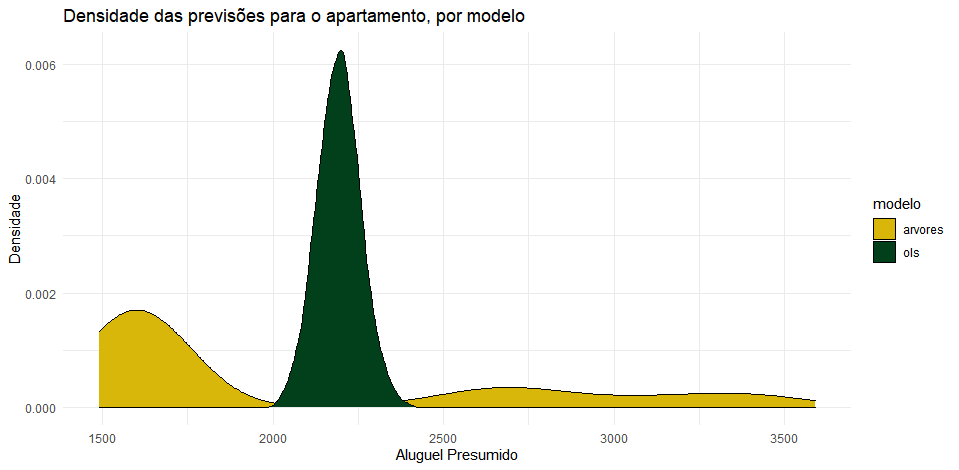
\includegraphics[scale = .40]{imagens/exemplo_var_arvores.png}
    \caption{A distribuição das previsões por classe de modelo. Elaboração própria.}
    \label{fig:arvore_var_ols}
\end{figure}
\end{frame}


\begin{frame}
Como lidar com isso? Uma maneira de mitigar a variância é treinar não só uma, mas várias árvores e usar a média de suas previsões como previsão final. Como árvores têm variância finita, a média da floresta tem distribuição normal e variância finita.

\begin{teo}[Lindenberg-Lévy]
Seja $(\textbf{X}_1, ..., \textbf{X}_n)$ uma amostra independente e identicamente distribuída com $\E[\textbf{X}_i] = \mu$ e $\V[\textbf{X}_i] = \sigma^2 < \infty$. Então:

\begin{align}
    \sqrt{n}\,(\bar{\textbf{X}_i }- \mu) \xrightarrow[n \to \infty]{d} N(0, \sigma^2)
\end{align}

\end{teo}
\end{frame}




\begin{frame}
Maneiras de mitigar a variância da floresta:

\begin{itemize}
    \item Treinar árvores \textit{rasas}, com poucas regras de classificação, portanto com menos variância
    \item Expor as árvores a subconjuntos dos dados (\textbf{bagging}, na literatura)
    \item Expor as árvores a um subconjunto das variáveis explicativas
\end{itemize}
\end{frame}



\begin{frame}
O que ainda não temos? Interpretabilidade. O modelo não entrega os efeitos marginais como em modelos lineares.



\begin{align}
    \frac{\partial \hat{y}}{\partial x_i} = \beta_i
\end{align}
\end{frame}


\begin{frame}
Uma abordagem é simular uma observação de referência e criar cópias adicionando pequenas variações na variável de interesse. Podemos treinar várias florestas e construir curvas de previsões. 

\begin{figure}[H]
    \centering
    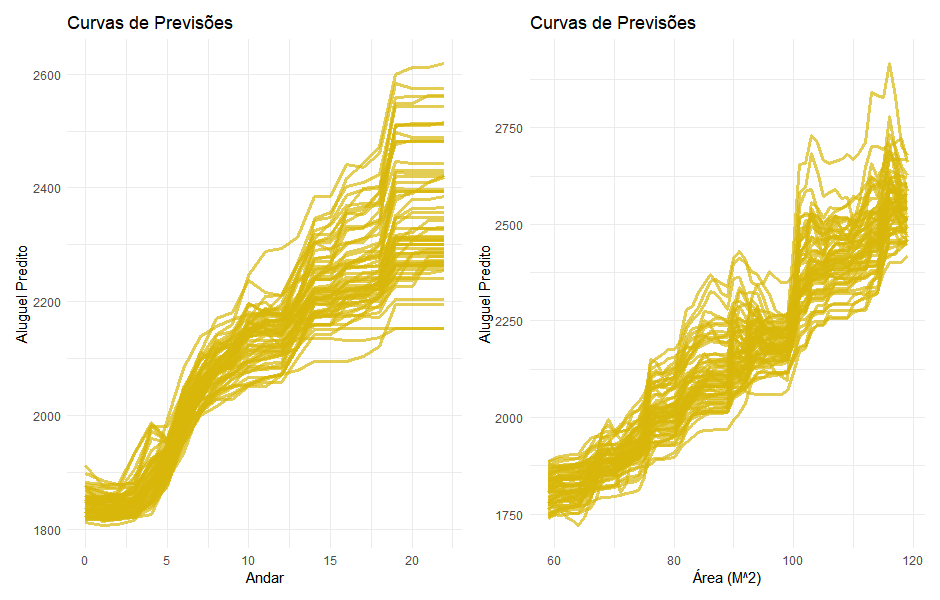
\includegraphics[scale = .25]{imagens/curvas_previsoes_rf.png}
    \caption{Curvas de previsões, uma para cada modelo. Elaboração própria.}
\end{figure}

\end{frame}







\begin{frame}

\end{frame}










\end{document}